\begin{frame}
\frametitle{XGBoost algorithm}

\begin{itemize}
    \small
    \item We used the XGBoost  (eXtreme Gradient Boosting) algorithm. It works by combining multiple weak predictive models to  create a stronger, more accurate model.
    \item XGboost uses multiple decision trees, each of which is built to reduce the residual error from the previous tree.
    \item The weight of each tree reduces as trees are added (to avoid over-fitting).
    \item The final prediction is the sum of the predictions of all the trees multiplied by their weights.

\end{itemize}

\begin{center}
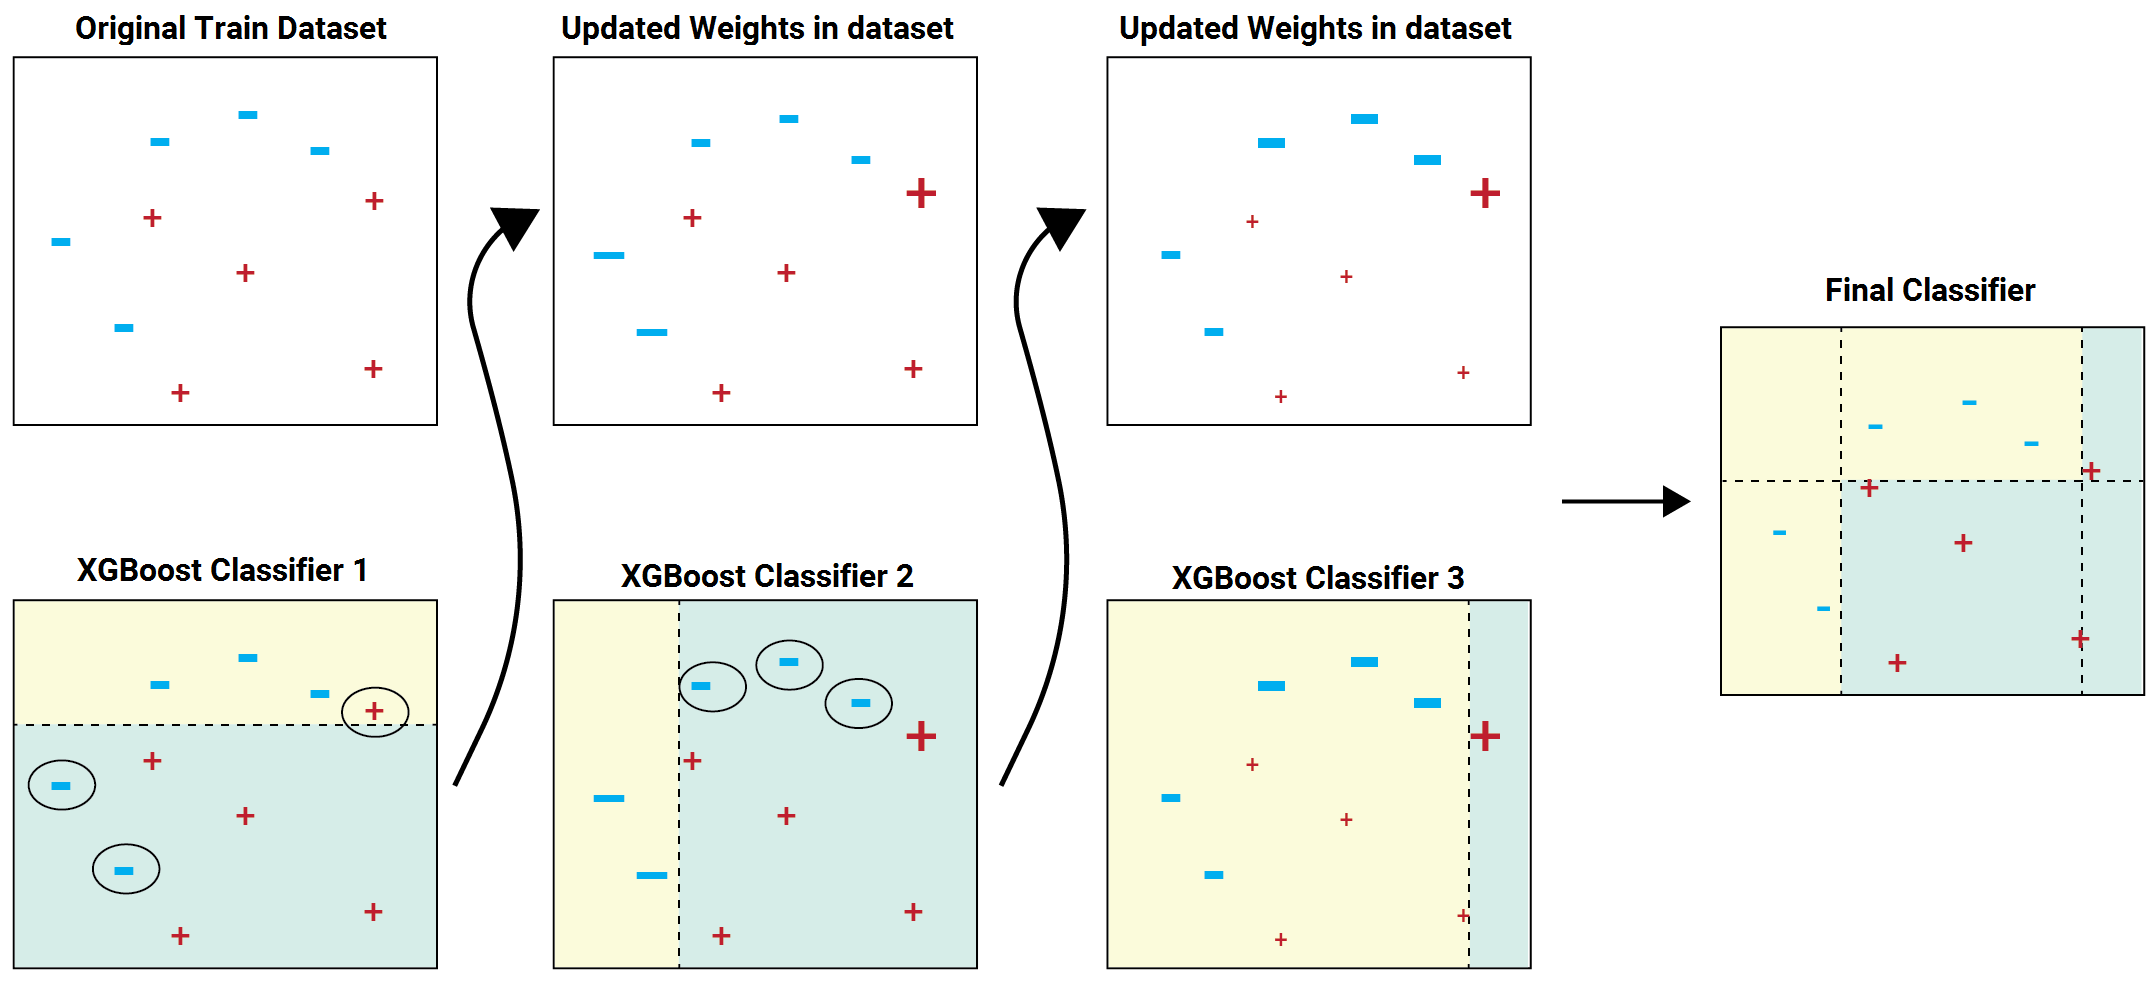
\includegraphics[width=0.75\textwidth]{./images/xgboost}
\end{center}

\tiny
Image from \url{https://blog.quantinsti.com/xgboost-python/}

\end{frame}